% Created by tikzDevice version 0.12.3 on 2020-01-25 19:17:02
% !TEX encoding = UTF-8 Unicode
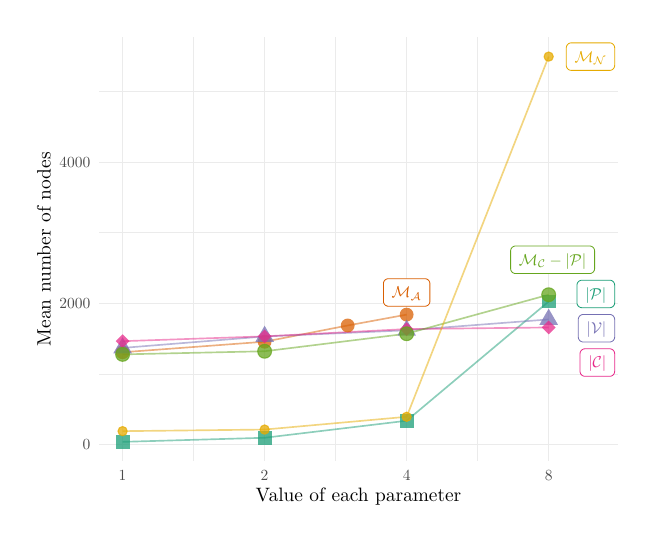
\begin{tikzpicture}[x=1pt,y=1pt]
\definecolor{fillColor}{RGB}{255,255,255}
\path[use as bounding box,fill=fillColor,fill opacity=0.00] (0,0) rectangle (216.81,176.16);
\begin{scope}
\path[clip] ( 25.78, 19.53) rectangle (213.31,172.66);
\definecolor{drawColor}{gray}{0.92}

\path[draw=drawColor,line width= 0.2pt,line join=round] ( 25.78, 51.08) --
	(213.31, 51.08);

\path[draw=drawColor,line width= 0.2pt,line join=round] ( 25.78,102.07) --
	(213.31,102.07);

\path[draw=drawColor,line width= 0.2pt,line join=round] ( 25.78,153.07) --
	(213.31,153.07);

\path[draw=drawColor,line width= 0.2pt,line join=round] ( 59.96, 19.53) --
	( 59.96,172.66);

\path[draw=drawColor,line width= 0.2pt,line join=round] (111.28, 19.53) --
	(111.28,172.66);

\path[draw=drawColor,line width= 0.2pt,line join=round] (162.60, 19.53) --
	(162.60,172.66);

\path[draw=drawColor,line width= 0.4pt,line join=round] ( 25.78, 25.58) --
	(213.31, 25.58);

\path[draw=drawColor,line width= 0.4pt,line join=round] ( 25.78, 76.58) --
	(213.31, 76.58);

\path[draw=drawColor,line width= 0.4pt,line join=round] ( 25.78,127.57) --
	(213.31,127.57);

\path[draw=drawColor,line width= 0.4pt,line join=round] ( 34.30, 19.53) --
	( 34.30,172.66);

\path[draw=drawColor,line width= 0.4pt,line join=round] ( 85.62, 19.53) --
	( 85.62,172.66);

\path[draw=drawColor,line width= 0.4pt,line join=round] (136.94, 19.53) --
	(136.94,172.66);

\path[draw=drawColor,line width= 0.4pt,line join=round] (188.26, 19.53) --
	(188.26,172.66);
\definecolor{drawColor}{RGB}{27,158,119}

\path[draw=drawColor,draw opacity=0.50,line width= 0.6pt,line join=round] ( 34.30, 26.49) --
	( 85.62, 27.97) --
	(136.94, 34.12) --
	(188.26, 77.20);
\definecolor{drawColor}{RGB}{217,95,2}

\path[draw=drawColor,draw opacity=0.50,line width= 0.6pt,line join=round] ( 34.30, 58.87) --
	( 85.62, 62.68) --
	(115.64, 68.55) --
	(136.94, 72.47);
\definecolor{drawColor}{RGB}{117,112,179}

\path[draw=drawColor,draw opacity=0.50,line width= 0.6pt,line join=round] ( 34.30, 60.44) --
	( 85.62, 64.58) --
	(136.94, 66.81) --
	(188.26, 70.73);
\definecolor{drawColor}{RGB}{231,41,138}

\path[draw=drawColor,draw opacity=0.50,line width= 0.6pt,line join=round] ( 34.30, 62.87) --
	( 85.62, 64.62) --
	(136.94, 67.25) --
	(188.26, 67.83);
\definecolor{drawColor}{RGB}{102,166,30}

\path[draw=drawColor,draw opacity=0.50,line width= 0.6pt,line join=round] ( 34.30, 58.10) --
	( 85.62, 59.23) --
	(136.94, 65.57) --
	(188.26, 79.66);
\definecolor{drawColor}{RGB}{230,171,2}

\path[draw=drawColor,draw opacity=0.50,line width= 0.6pt,line join=round] ( 34.30, 30.36) --
	( 85.62, 30.94) --
	(136.94, 35.55) --
	(188.26,165.70);
\definecolor{fillColor}{RGB}{27,158,119}

\path[fill=fillColor,fill opacity=0.75] ( 31.81, 23.99) --
	( 36.80, 23.99) --
	( 36.80, 28.99) --
	( 31.81, 28.99) --
	cycle;

\path[fill=fillColor,fill opacity=0.75] ( 83.13, 25.47) --
	( 88.12, 25.47) --
	( 88.12, 30.46) --
	( 83.13, 30.46) --
	cycle;

\path[fill=fillColor,fill opacity=0.75] (134.45, 31.63) --
	(139.44, 31.63) --
	(139.44, 36.62) --
	(134.45, 36.62) --
	cycle;

\path[fill=fillColor,fill opacity=0.75] (185.77, 74.70) --
	(190.76, 74.70) --
	(190.76, 79.69) --
	(185.77, 79.69) --
	cycle;
\definecolor{fillColor}{RGB}{217,95,2}

\path[fill=fillColor,fill opacity=0.75] ( 34.30, 58.87) circle (  2.50);

\path[fill=fillColor,fill opacity=0.75] ( 85.62, 62.68) circle (  2.50);

\path[fill=fillColor,fill opacity=0.75] (115.64, 68.55) circle (  2.50);

\path[fill=fillColor,fill opacity=0.75] (136.94, 72.47) circle (  2.50);
\definecolor{fillColor}{RGB}{117,112,179}

\path[fill=fillColor,fill opacity=0.75] ( 34.30, 64.32) --
	( 37.67, 58.50) --
	( 30.94, 58.50) --
	cycle;

\path[fill=fillColor,fill opacity=0.75] ( 85.62, 68.46) --
	( 88.99, 62.64) --
	( 82.26, 62.64) --
	cycle;

\path[fill=fillColor,fill opacity=0.75] (136.94, 70.70) --
	(140.31, 64.87) --
	(133.58, 64.87) --
	cycle;

\path[fill=fillColor,fill opacity=0.75] (188.26, 74.62) --
	(191.63, 68.79) --
	(184.90, 68.79) --
	cycle;
\definecolor{fillColor}{RGB}{231,41,138}

\path[fill=fillColor,fill opacity=0.75] ( 31.81, 62.87) --
	( 34.30, 65.37) --
	( 36.80, 62.87) --
	( 34.30, 60.37) --
	cycle;

\path[fill=fillColor,fill opacity=0.75] ( 83.13, 64.62) --
	( 85.62, 67.11) --
	( 88.12, 64.62) --
	( 85.62, 62.12) --
	cycle;

\path[fill=fillColor,fill opacity=0.75] (134.45, 67.25) --
	(136.94, 69.74) --
	(139.44, 67.25) --
	(136.94, 64.75) --
	cycle;

\path[fill=fillColor,fill opacity=0.75] (185.77, 67.83) --
	(188.26, 70.32) --
	(190.76, 67.83) --
	(188.26, 65.33) --
	cycle;
\definecolor{drawColor}{RGB}{102,166,30}
\definecolor{fillColor}{RGB}{102,166,30}

\path[draw=drawColor,draw opacity=0.75,line width= 0.4pt,line join=round,line cap=round,fill=fillColor,fill opacity=0.75] ( 34.30, 58.10) circle (  2.50);

\path[draw=drawColor,draw opacity=0.75,line width= 0.4pt,line join=round,line cap=round,fill=fillColor,fill opacity=0.75] ( 85.62, 59.23) circle (  2.50);

\path[draw=drawColor,draw opacity=0.75,line width= 0.4pt,line join=round,line cap=round,fill=fillColor,fill opacity=0.75] (136.94, 65.57) circle (  2.50);

\path[draw=drawColor,draw opacity=0.75,line width= 0.4pt,line join=round,line cap=round,fill=fillColor,fill opacity=0.75] (188.26, 79.66) circle (  2.50);
\definecolor{drawColor}{RGB}{230,171,2}
\definecolor{fillColor}{RGB}{230,171,2}

\path[draw=drawColor,draw opacity=0.75,line width= 0.4pt,line join=round,line cap=round,fill=fillColor,fill opacity=0.75] ( 34.30, 30.36) circle (  1.67);

\path[draw=drawColor,draw opacity=0.75,line width= 0.4pt,line join=round,line cap=round,fill=fillColor,fill opacity=0.75] ( 85.62, 30.94) circle (  1.67);

\path[draw=drawColor,draw opacity=0.75,line width= 0.4pt,line join=round,line cap=round,fill=fillColor,fill opacity=0.75] (136.94, 35.55) circle (  1.67);

\path[draw=drawColor,draw opacity=0.75,line width= 0.4pt,line join=round,line cap=round,fill=fillColor,fill opacity=0.75] (188.26,165.70) circle (  1.67);
\end{scope}
\begin{scope}
\path[clip] ( 25.78, 19.53) rectangle (213.31,172.66);

\path[] (198.49, 79.80) -- (188.26, 77.20);
\definecolor{drawColor}{RGB}{27,158,119}
\definecolor{fillColor}{RGB}{255,255,255}

\path[draw=drawColor,line width= 0.3pt,line join=round,line cap=round,fill=fillColor] (200.30, 74.97) --
	(210.30, 74.97) --
	(210.23, 74.97) --
	(210.52, 74.98) --
	(210.80, 75.04) --
	(211.07, 75.14) --
	(211.33, 75.29) --
	(211.55, 75.47) --
	(211.74, 75.69) --
	(211.90, 75.94) --
	(212.01, 76.20) --
	(212.08, 76.49) --
	(212.11, 76.78) --
	(212.11, 76.78) --
	(212.11, 83.11) --
	(212.11, 83.11) --
	(212.08, 83.40) --
	(212.01, 83.68) --
	(211.90, 83.94) --
	(211.74, 84.19) --
	(211.55, 84.41) --
	(211.33, 84.59) --
	(211.07, 84.74) --
	(210.80, 84.84) --
	(210.52, 84.90) --
	(210.30, 84.91) --
	(200.30, 84.91) --
	(200.52, 84.90) --
	(200.23, 84.91) --
	(199.94, 84.88) --
	(199.66, 84.79) --
	(199.40, 84.67) --
	(199.16, 84.50) --
	(198.95, 84.30) --
	(198.77, 84.07) --
	(198.64, 83.81) --
	(198.55, 83.54) --
	(198.50, 83.25) --
	(198.49, 83.11) --
	(198.49, 76.78) --
	(198.50, 76.92) --
	(198.50, 76.63) --
	(198.55, 76.34) --
	(198.64, 76.07) --
	(198.77, 75.81) --
	(198.95, 75.58) --
	(199.16, 75.38) --
	(199.40, 75.21) --
	(199.66, 75.09) --
	(199.94, 75.01) --
	(200.23, 74.97) --
	cycle;
\end{scope}
\begin{scope}
\path[clip] ( 25.78, 19.53) rectangle (213.31,172.66);
\definecolor{drawColor}{RGB}{27,158,119}

\node[text=drawColor,anchor=base,inner sep=0pt, outer sep=0pt, scale=  0.57] at (205.30, 77.98) {$|\mathcal{P}|$};
\end{scope}
\begin{scope}
\path[clip] ( 25.78, 19.53) rectangle (213.31,172.66);

\path[] (198.97, 67.74) -- (188.26, 70.73);
\definecolor{drawColor}{RGB}{117,112,179}
\definecolor{fillColor}{RGB}{255,255,255}

\path[draw=drawColor,line width= 0.3pt,line join=round,line cap=round,fill=fillColor] (200.77, 62.58) --
	(210.30, 62.58) --
	(210.23, 62.58) --
	(210.52, 62.59) --
	(210.80, 62.65) --
	(211.07, 62.75) --
	(211.33, 62.90) --
	(211.55, 63.08) --
	(211.74, 63.30) --
	(211.90, 63.54) --
	(212.01, 63.81) --
	(212.08, 64.09) --
	(212.11, 64.38) --
	(212.11, 64.38) --
	(212.11, 70.71) --
	(212.11, 70.71) --
	(212.08, 71.00) --
	(212.01, 71.29) --
	(211.90, 71.55) --
	(211.74, 71.80) --
	(211.55, 72.02) --
	(211.33, 72.20) --
	(211.07, 72.35) --
	(210.80, 72.45) --
	(210.52, 72.51) --
	(210.30, 72.52) --
	(200.77, 72.52) --
	(200.99, 72.51) --
	(200.70, 72.52) --
	(200.41, 72.48) --
	(200.13, 72.40) --
	(199.87, 72.28) --
	(199.63, 72.11) --
	(199.42, 71.91) --
	(199.25, 71.68) --
	(199.11, 71.42) --
	(199.02, 71.15) --
	(198.97, 70.86) --
	(198.97, 70.71) --
	(198.97, 64.38) --
	(198.97, 64.53) --
	(198.97, 64.24) --
	(199.02, 63.95) --
	(199.11, 63.68) --
	(199.25, 63.42) --
	(199.42, 63.19) --
	(199.63, 62.99) --
	(199.87, 62.82) --
	(200.13, 62.70) --
	(200.41, 62.61) --
	(200.70, 62.58) --
	cycle;
\end{scope}
\begin{scope}
\path[clip] ( 25.78, 19.53) rectangle (213.31,172.66);
\definecolor{drawColor}{RGB}{117,112,179}

\node[text=drawColor,anchor=base,inner sep=0pt, outer sep=0pt, scale=  0.57] at (205.54, 65.59) {$|\mathcal{V}|$};
\end{scope}
\begin{scope}
\path[clip] ( 25.78, 19.53) rectangle (213.31,172.66);

\path[] (199.59, 56.31) -- (188.26, 67.83);
\definecolor{drawColor}{RGB}{231,41,138}
\definecolor{fillColor}{RGB}{255,255,255}

\path[draw=drawColor,line width= 0.3pt,line join=round,line cap=round,fill=fillColor] (201.40, 50.18) --
	(210.30, 50.18) --
	(210.23, 50.18) --
	(210.52, 50.19) --
	(210.80, 50.25) --
	(211.07, 50.35) --
	(211.33, 50.50) --
	(211.55, 50.68) --
	(211.74, 50.90) --
	(211.90, 51.15) --
	(212.01, 51.41) --
	(212.08, 51.70) --
	(212.11, 51.99) --
	(212.11, 51.99) --
	(212.11, 58.31) --
	(212.11, 58.31) --
	(212.08, 58.60) --
	(212.01, 58.89) --
	(211.90, 59.15) --
	(211.74, 59.40) --
	(211.55, 59.62) --
	(211.33, 59.80) --
	(211.07, 59.95) --
	(210.80, 60.05) --
	(210.52, 60.11) --
	(210.30, 60.12) --
	(201.40, 60.12) --
	(201.62, 60.11) --
	(201.33, 60.12) --
	(201.04, 60.08) --
	(200.76, 60.00) --
	(200.50, 59.88) --
	(200.26, 59.71) --
	(200.05, 59.51) --
	(199.87, 59.28) --
	(199.74, 59.02) --
	(199.65, 58.75) --
	(199.60, 58.46) --
	(199.59, 58.31) --
	(199.59, 51.99) --
	(199.60, 52.13) --
	(199.60, 51.84) --
	(199.65, 51.55) --
	(199.74, 51.28) --
	(199.87, 51.02) --
	(200.05, 50.79) --
	(200.26, 50.59) --
	(200.50, 50.42) --
	(200.76, 50.30) --
	(201.04, 50.22) --
	(201.33, 50.18) --
	cycle;
\end{scope}
\begin{scope}
\path[clip] ( 25.78, 19.53) rectangle (213.31,172.66);
\definecolor{drawColor}{RGB}{231,41,138}

\node[text=drawColor,anchor=base,inner sep=0pt, outer sep=0pt, scale=  0.57] at (205.85, 53.19) {$|\mathcal{C}|$};
\end{scope}
\begin{scope}
\path[clip] ( 25.78, 19.53) rectangle (213.31,172.66);

\path[] (189.67, 87.32) -- (188.26, 79.66);
\definecolor{drawColor}{RGB}{102,166,30}
\definecolor{fillColor}{RGB}{255,255,255}

\path[draw=drawColor,line width= 0.3pt,line join=round,line cap=round,fill=fillColor] (176.31, 87.32) --
	(203.05, 87.32) --
	(202.98, 87.32) --
	(203.27, 87.33) --
	(203.56, 87.39) --
	(203.83, 87.49) --
	(204.08, 87.64) --
	(204.31, 87.82) --
	(204.50, 88.04) --
	(204.65, 88.28) --
	(204.77, 88.55) --
	(204.84, 88.83) --
	(204.86, 89.12) --
	(204.86, 89.12) --
	(204.86, 95.45) --
	(204.86, 95.45) --
	(204.84, 95.74) --
	(204.77, 96.03) --
	(204.65, 96.29) --
	(204.50, 96.54) --
	(204.31, 96.76) --
	(204.08, 96.94) --
	(203.83, 97.09) --
	(203.56, 97.19) --
	(203.27, 97.25) --
	(203.05, 97.26) --
	(176.31, 97.26) --
	(176.53, 97.25) --
	(176.24, 97.26) --
	(175.95, 97.22) --
	(175.67, 97.14) --
	(175.41, 97.02) --
	(175.17, 96.85) --
	(174.96, 96.65) --
	(174.79, 96.42) --
	(174.65, 96.16) --
	(174.56, 95.89) --
	(174.51, 95.60) --
	(174.51, 95.45) --
	(174.51, 89.12) --
	(174.51, 89.27) --
	(174.51, 88.98) --
	(174.56, 88.69) --
	(174.65, 88.42) --
	(174.79, 88.16) --
	(174.96, 87.93) --
	(175.17, 87.72) --
	(175.41, 87.56) --
	(175.67, 87.44) --
	(175.95, 87.35) --
	(176.24, 87.32) --
	cycle;
\end{scope}
\begin{scope}
\path[clip] ( 25.78, 19.53) rectangle (213.31,172.66);
\definecolor{drawColor}{RGB}{102,166,30}

\node[text=drawColor,anchor=base,inner sep=0pt, outer sep=0pt, scale=  0.57] at (189.68, 90.33) {$\mathcal{M}_{\mathcal{C}}-|\mathcal{P}|$};
\end{scope}
\begin{scope}
\path[clip] ( 25.78, 19.53) rectangle (213.31,172.66);

\path[] (194.64,165.70) -- (188.26,165.70);
\definecolor{drawColor}{RGB}{230,171,2}
\definecolor{fillColor}{RGB}{255,255,255}

\path[draw=drawColor,line width= 0.3pt,line join=round,line cap=round,fill=fillColor] (196.44,160.73) --
	(210.30,160.73) --
	(210.23,160.73) --
	(210.52,160.74) --
	(210.80,160.80) --
	(211.07,160.90) --
	(211.33,161.05) --
	(211.55,161.23) --
	(211.74,161.45) --
	(211.90,161.69) --
	(212.01,161.96) --
	(212.08,162.24) --
	(212.11,162.53) --
	(212.11,162.53) --
	(212.11,168.86) --
	(212.11,168.86) --
	(212.08,169.15) --
	(212.01,169.43) --
	(211.90,169.70) --
	(211.74,169.95) --
	(211.55,170.16) --
	(211.33,170.35) --
	(211.07,170.49) --
	(210.80,170.60) --
	(210.52,170.66) --
	(210.30,170.67) --
	(196.44,170.67) --
	(196.66,170.66) --
	(196.37,170.67) --
	(196.08,170.63) --
	(195.80,170.55) --
	(195.54,170.43) --
	(195.30,170.26) --
	(195.09,170.06) --
	(194.92,169.83) --
	(194.78,169.57) --
	(194.69,169.29) --
	(194.64,169.01) --
	(194.64,168.86) --
	(194.64,162.53) --
	(194.64,162.68) --
	(194.64,162.39) --
	(194.69,162.10) --
	(194.78,161.82) --
	(194.92,161.57) --
	(195.09,161.34) --
	(195.30,161.13) --
	(195.54,160.97) --
	(195.80,160.84) --
	(196.08,160.76) --
	(196.37,160.73) --
	cycle;
\end{scope}
\begin{scope}
\path[clip] ( 25.78, 19.53) rectangle (213.31,172.66);
\definecolor{drawColor}{RGB}{230,171,2}

\node[text=drawColor,anchor=base,inner sep=0pt, outer sep=0pt, scale=  0.57] at (203.37,163.74) {$\mathcal{M}_{\mathcal{N}}$};
\end{scope}
\begin{scope}
\path[clip] ( 25.78, 19.53) rectangle (213.31,172.66);
\definecolor{drawColor}{RGB}{217,95,2}
\definecolor{fillColor}{RGB}{255,255,255}

\path[draw=drawColor,line width= 0.3pt,line join=round,line cap=round,fill=fillColor] (130.35, 75.50) --
	(143.54, 75.50) --
	(143.46, 75.51) --
	(143.75, 75.52) --
	(144.04, 75.58) --
	(144.31, 75.68) --
	(144.56, 75.82) --
	(144.79, 76.01) --
	(144.98, 76.23) --
	(145.14, 76.47) --
	(145.25, 76.74) --
	(145.32, 77.02) --
	(145.34, 77.31) --
	(145.34, 77.31) --
	(145.34, 83.64) --
	(145.34, 83.64) --
	(145.32, 83.93) --
	(145.25, 84.21) --
	(145.14, 84.48) --
	(144.98, 84.72) --
	(144.79, 84.94) --
	(144.56, 85.13) --
	(144.31, 85.27) --
	(144.04, 85.37) --
	(143.75, 85.43) --
	(143.54, 85.45) --
	(130.35, 85.45) --
	(130.57, 85.43) --
	(130.28, 85.44) --
	(129.99, 85.41) --
	(129.71, 85.33) --
	(129.45, 85.20) --
	(129.21, 85.04) --
	(129.00, 84.84) --
	(128.83, 84.61) --
	(128.69, 84.35) --
	(128.60, 84.07) --
	(128.55, 83.78) --
	(128.55, 83.64) --
	(128.55, 77.31) --
	(128.55, 77.46) --
	(128.55, 77.17) --
	(128.60, 76.88) --
	(128.69, 76.60) --
	(128.83, 76.35) --
	(129.00, 76.11) --
	(129.21, 75.91) --
	(129.45, 75.75) --
	(129.71, 75.62) --
	(129.99, 75.54) --
	(130.28, 75.51) --
	cycle;
\end{scope}
\begin{scope}
\path[clip] ( 25.78, 19.53) rectangle (213.31,172.66);
\definecolor{drawColor}{RGB}{217,95,2}

\node[text=drawColor,anchor=base,inner sep=0pt, outer sep=0pt, scale=  0.57] at (136.94, 78.52) {$\mathcal{M}_{\mathcal{A}}$};
\end{scope}
\begin{scope}
\path[clip] (  0.00,  0.00) rectangle (216.81,176.16);
\definecolor{drawColor}{gray}{0.30}

\node[text=drawColor,anchor=base east,inner sep=0pt, outer sep=0pt, scale=  0.56] at ( 22.63, 23.65) {0};

\node[text=drawColor,anchor=base east,inner sep=0pt, outer sep=0pt, scale=  0.56] at ( 22.63, 74.65) {2000};

\node[text=drawColor,anchor=base east,inner sep=0pt, outer sep=0pt, scale=  0.56] at ( 22.63,125.64) {4000};
\end{scope}
\begin{scope}
\path[clip] (  0.00,  0.00) rectangle (216.81,176.16);
\definecolor{drawColor}{gray}{0.30}

\node[text=drawColor,anchor=base,inner sep=0pt, outer sep=0pt, scale=  0.56] at ( 34.30, 12.52) {1};

\node[text=drawColor,anchor=base,inner sep=0pt, outer sep=0pt, scale=  0.56] at ( 85.62, 12.52) {2};

\node[text=drawColor,anchor=base,inner sep=0pt, outer sep=0pt, scale=  0.56] at (136.94, 12.52) {4};

\node[text=drawColor,anchor=base,inner sep=0pt, outer sep=0pt, scale=  0.56] at (188.26, 12.52) {8};
\end{scope}
\begin{scope}
\path[clip] (  0.00,  0.00) rectangle (216.81,176.16);
\definecolor{drawColor}{RGB}{0,0,0}

\node[text=drawColor,anchor=base,inner sep=0pt, outer sep=0pt, scale=  0.70] at (119.54,  4.86) {Value of each parameter};
\end{scope}
\begin{scope}
\path[clip] (  0.00,  0.00) rectangle (216.81,176.16);
\definecolor{drawColor}{RGB}{0,0,0}

\node[text=drawColor,rotate= 90.00,anchor=base,inner sep=0pt, outer sep=0pt, scale=  0.70] at (  8.32, 96.09) {Mean number of nodes};
\end{scope}
\end{tikzpicture}
